\chapter{PRELIMINARIES AND NOTIONS}

The major perspective of this thesis is to extend the applicability of the golden-standard \acrshort{vslam} paradigms for outdoor robotic usage and finally achieves life-long autonomy.
In other words, our work is to robustify the estimation process of the {\em front-end} and {\em back-end} of \acrshort{vslam} system.
Thereby, understanding the underlying logic behind camera motion and scene structure estimation is of paramount importance.  
In this section, a brief review of the most relevant preliminaries and notions, e.g. \acrshort{map} estimation, energy functions, optimization over Lie-manifold, and problem definition of the localization and mapping are briefly described for a better understanding of our work.

\section{Maximum A Posterior Estimation} 
\label{sec:preliminaries_map}
Underlying all formulations of \acrshort{vslam} is a probabilistic model that inputs noisy measurements $\mathbf{Z} = \{ z_k \ | \ k = 1, 2, \cdot, K \}$ and outputs hidden model variables $\mathbf{X}$ by solving a batch of (non)linear functions $z_k = h(\mathbf{X}_k) + \epsilon_k$, where $\mathbf{X}_k \subset \mathbf{X}$ is a subset of hidden variables and $h(\cdot)$ is a task-dependent observation model.  
Typically, it is solved by \acrshort{map} estimation that computes the model $\mathbf{X}$ to realize the maximum of posterior from the actual measurements $\mathbf{Z}$:
\begin{equation} \label{eq:preliminaries_probmodel}
\begin{split}
\mathbf{X}^* &:=  \argmax_{\mathbf{X}} Pr(\mathbf{X} | \mathbf{Z}) \\
&:= \argmax_{\mathbf{X}} Pr(\mathbf{X}) Pr(\mathbf{Z} | \mathbf{X}) 
\end{split}
\end{equation} 
where $Pr(\mathbf{Z} | \mathbf{X})$ is the likelihood of the measurements $\mathbf{Z}$ given state $\mathbf{X}$ and $Pr(\mathbf{X})$ is the prior probability. 
Assuming (1) each measurement $z_k \in \mathbf{Z}$ is independent with each other and (2) all underlying model conform Gaussian noise distributions, the \acrshort{map} estimation problem can be re-factorized to be a (non)linear least square optimization problem:
\begin{equation} \label{eq:preliminaries_lsmodel}
\begin{split}
\mathbf{X}^* &= \argmax_{\mathbf{X}} \sum_{k} Pr(\mathbf{X}_k) Pr(z_k | \mathbf{X}_k) \\
&=  \argmin_{\mathbf{X}} -\log \sum_{k} Pr(\mathbf{X}_k) Pr(z_k | \mathbf{X}_k) \\
&= \argmin_{\mathbf{X}} \sum_{k} w_k \| z_k - h(\mathbf{X}_k) \|_{\Omega}
\end{split}
\end{equation} 
where $\Omega$ denotes type of normal function that is tightly related with the noise model of selection.
It could be either well-known $l1$-, $l2$-norm, or robust Huber loss functions.
Typically, the measurements $z_k$ have lower dimensions compared with state variables $\mathbf{X}_k$, which requires multiple observations to recover a unique solution for the estimates.
 
\section{Energy Formulations for Indirect and Direct Methods} 
\label{sec:preliminaries_energy}
Let us consider a reference frame, an acquired image $I_{r}: \Omega \rightarrow \mathbb{R}$ and its inverse depth map  $D_{r}: \Omega \rightarrow \mathbb{R}^{+}$, where $\Omega \subset \mathbb{R}^2$ is the image domain. 
A 3D scene point $\mathbf{P} = (x, y, z)^{T}$ is parameterized by its inverse depth $d = z^{-1}$ in the reference frame instead of the conventional 3 unknowns. Each pixel in the reference frame $\mathbf{p} = (u,v)^T \in \Omega$ can be back-projected into 3D world using the back-projection function $\mathbf{P} = \pi^{-1}(\mathbf{p})$. 
Inversely, the 3D projective warp function $\mathbf{p} = \pi(\mathbf{P})$ can project 3D point onto image space. 

A 3D rigid body transformation $\mathbf{G} \in SE(3)$ can be generally divided into a 3D rigid body rotation $\mathbf{R} \in SO(3)$ and translation $\mathbf{t} \in \mathbb{R}^3$. 
The relative transformation $\mathbf{G}_{rk}$ in the optimization framework can be initialized from their individual global poses as $\mathbf{G}_{rk} = \mathbf{G}_{wr}^{-1}\mathbf{G}_{wk}$.  

Given arbitrary pixel selector $\mathit{S}(\cdot)$, the group of selected pixels $\mathit{S}_r$ extracted from the reference image can be expressed as:
\begin{equation} \label{eq:preliminaries_selector}
\mathit{S}_r =  \left \{ \mathbf{p}_r \right \} = \mathit{S}(I_r) 
\end{equation} 
Each selected pixel $ \mathbf{p}_r \in \mathit{S}_{r}$ are subsequently projected to current frame $k$ as:
\begin{equation} \label{eq:preliminaries_pointproj}
 \mathbf{p}_{kr} =  \pi ( \mathbf{R}_{kr}\pi^{-1}(\mathbf{p}_r,D_{r}(\mathbf{p}_r) )+\mathbf{t}_{kr} ) 
\end{equation} 

\begin{figure}[t]
    \centering
	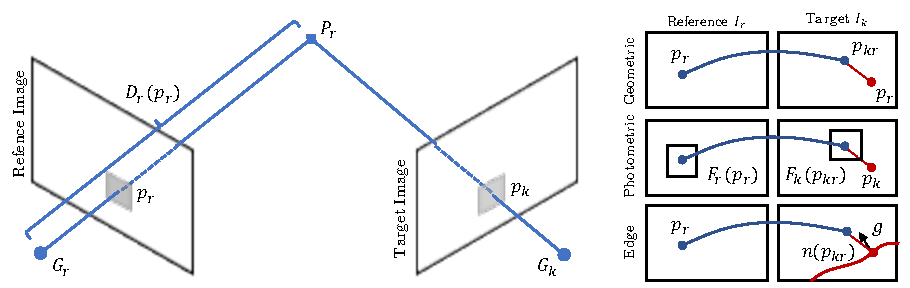
\includegraphics[width=1.0\textwidth]{figures/prelim/reprojection.pdf}
	\caption[Point Reprojection and Energy Function Designs]{\textbf{Point Reprojection and Energy Function Designs.} Geometric (\textbf{Right-Top}), photometric (\textbf{Right-Mid}), and edge-based (\textbf{Right-Bottom}) \acrshort{vslam} paradigms.
	\label{fig:preliminaries_energy}}
\end{figure} 
 

The generalized photometric error $E_{kr}^{\mathcal{P}}$, edge alignment error $E_{kr}^{\mathcal{E}}$, and reprojection error $E_{kr}^{\mathcal{R}}$ from reference frame to frame $k$ can be generally written as:
\begin{align} 
E_{kr}^{\mathcal{R}} &:=  \sum_{\mathbf{p}_{r} \in \mathit{S}_r^{\mathcal{R}} } w_{\mathbf{p}_r}^{\mathcal{R}} \Vert \mathbf{p}_{kr} - \mathbf{p}_{k} \Vert_{\gamma}  \label{eq:preliminaries_reprojectionerror} \\
E_{kr}^{\mathcal{P}} &:= \sum_{\mathbf{p}_r \in \mathit{S}_r^{\mathcal{P}}} w_{\mathbf{p}_r}^{\mathcal{P}} \Vert F_{k} ( \mathbf{p}_{kr}) - F_{r}(\mathbf{p}_r) \Vert_{\gamma} \label{eq:preliminaries_photometricerror} \\ 
E_{kr}^{\mathcal{E}} &:=  \sum_{\mathbf{p}_{r} \in \mathit{S}_r^{\mathcal{E}} } w_{\mathbf{p}_r}^{\mathcal{E}} \Vert \mathbf{g}(\mathbf{p}_{kr} - \mathit{n}(\mathbf{p}_{kr})) \Vert_{\gamma}  \label{eq:preliminaries_edgeerror}
\end{align}
where $w_{\mathbf{p}_r}$ is the weight assigned for each selected pixel from $S_r$ in reference frame, and $\Vert \cdot \Vert_{\gamma}$ is the Huber norm. 
Specifically for each formulation, $\left \{ \mathbf{p}_{r},\mathbf{p}_{k} \right \}$ is a pair of matched points between reference image and image $k$, 
$F(\cdot)$ represents any representation calculated from Image $I$, such as intensity, gradient or some dense descriptors, 
$\mathit{n}(\mathbf{p}_{kr})$ represents the nearest neighbor of the projected edge pixel $\mathbf{p}_{kr}$ in current frame $k$ using the Euclidean distance metric, 
$\mathbf{g}$ represents the normal direction of edge points that is usually approximated using gradient direction of grey-scale image patch. 


For real-time performance, the optimization is usually done within a sliding window of keyframes, where the full errors over all frames and points within this window are optimized:
\begin{equation} \label{eq:preliminaries_opt}
E_{opt} = \sum_{(r,k)\in \mathit{W}} E_{kr}
\end{equation} 
where $\mathit{W}$ denotes the sliding window for local optimization. 
 
\section{Optimization in Lie-Manifold}
\label{sec:preliminaries_optimization}

\begin{figure}[t]
    \centering
	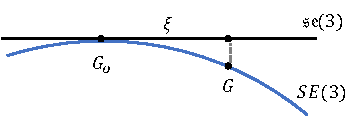
\includegraphics[width=0.5\textwidth]{figures/prelim/liegroup.pdf}
	\caption[Optimization in Lie-Manifold]{\textbf{Optimization in Lie-Manifold.} The blue curve denotes the parameter space in $SE(3)$, and black curve represents the corresponding rangent-space in $\mathfrak{se}(3)$ around $\mathbf{G}_0$. At each optimization iteration, we compute the update step $\xi$ and merge it back to $G_0$ through exponential mapping.
	\label{fig:preliminaries_liegroup}}
\end{figure} 

The formulated minimization problem is commonly solved via successive linearization, e.g. Gauss-Newton or the Levengerg-Marquardt methods. 
Such inverse compositional methods can be seamlessly generalized to variables on smooth Lie-manifolds. 
The corresponding Lie Group component $\xi \in \mathfrak{se}(3)$ is introduced to represent the 6-DoF camera pose, where this element can be mapped to $\mathbf{G} \in SE(3)$ through the exponential mapping as:
\begin{equation} \label{eq:preliminaries_expmapping}
\mathbf{G} = exp_{\mathfrak{se}(3)}(\xi)
\end{equation}
and the update rule in Lie Manifold can be performed through exponential mapping and matrix multiplication as:
\begin{equation} \label{eq:preliminaries_expaddition}
\mathbf{G}_{ik} = \mathbf{G}_{ij} \oplus \xi_{jk}  = \mathbf{G}_{ij} \cdot exp_{\mathfrak{se}(3)}(\xi_{jk})
\end{equation}

Note that the key insight of modern \acrshort{vslam} estimation is that the Jacobian and Hessian matrix formulated by the linearized energy functions is sparse, which enables fast linear solver, e.g. QR and Cholesky, to be involved for real-time performance.
Thereby, the optimization problem associated with \acrshort{vslam} can be seen as a large but sparse linear algebra, which can be efficiently solved through CHOLMOD AND SuiteSparseQR open-source solvers. 


\section{Optimization for Localization and Mapping}
\label{sec:preliminaries_locmap}
Recall that \acrshort{vslam} {\em back-end} is essentially a \acrshort{map} dual estimation problems. 
It treats relative camera poses $\mathbf{G}$ and scene structure $D$ within a pre-defined sliding window as optimization parameters.
Thereby, the optimizatin problem can be expressed as follows:
\begin{equation} \label{eq:preliminaries_mappingoptimization}
\mathbf{G}^*, D^* = \argmin_{\mathbf{G}, D} \sum_{(r,k)\in \mathit{W}} E_{kr}(\mathbf{G}_{rk}, D_r)
\end{equation} 
where $\mathbf{G}_{rk} \subset \mathbf{G}$ and $D_r \subset D$ are the subset of full optimization parameters within the optimization window $\mathit{W}$.

It worth noting that the above-mentioned optimization problem is highly nonlinear due to the invloved rotation components, which makes the initialization of states ultra important to prevent them arriving at local minimas during optimization.
It is such needs breeding the incremental pose initialization algorithm, namely camera localization.
The localization algorithm usually temporally fix the scene structures of reference frame $D_r$, and incrementally infer the relative camera pose $\mathbf{G}_{rk}$ from refencek keyframe to current frame:
\begin{equation} \label{eq:preliminaries_locoptimization}
\mathbf{G}_{rk}^* = \argmin_{\mathbf{G}_{rk}} \ E_{kr}(\mathbf{G}_{rk})
\end{equation} 

In conjunction with it, the scene structure initialization algorithms, e.g. DLT-based point triangulation or inverse depth filtering, are also deliberately designed for reliable joint optimization.
Although this step is usually achieved through linear approximation or nonlinear filtering, the optimization formulation is also provided here for completeness:
\begin{equation} \label{eq:preliminaries_dualoptimization}
D_{r}^* = \argmin_{D_{r}} \sum_{k \in near(r)} E_{kr}(D_{r})
\end{equation} 
where $near(r)$ is a subset of frames that is spatially or temporally near the current keyframe for depth initialization. 